\documentclass{article}
\usepackage{tikz}
\usetikzlibrary{arrows.meta}

\begin{document}

\begin{figure}[h]
    \centering
    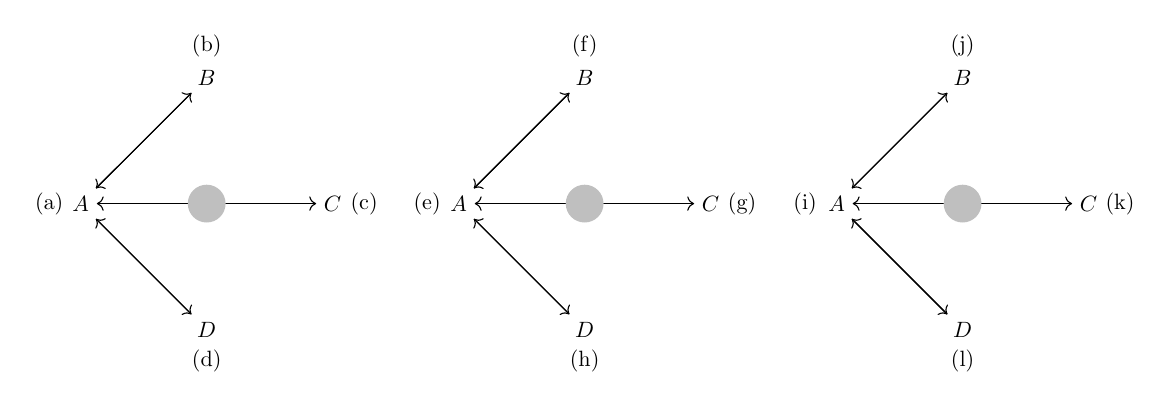
\begin{tikzpicture}[scale=0.8, every node/.style={transform shape}]
        % Define nodes
        \node (A) at (-2, 0) {$A$};
        \node (B) at (0, 2) {$B$};
        \node (C) at (2, 0) {$C$};
        \node (D) at (0, -2) {$D$};
        
        % Draw edges with arrows
        \draw[->] (A) -- (B);
        \draw[->] (A) -- (C);
        \draw[->] (A) -- (D);
        \draw[->] (B) -- (A);
        \draw[->] (C) -- (A);
        \draw[->] (D) -- (A);
        
        % Highlight the central node
        \fill[gray!50] (0, 0) circle (0.3cm);
        
        % Add labels for clarity
        \node at (-2.5, 0) {(a)};
        \node at (0, 2.5) {(b)};
        \node at (2.5, 0) {(c)};
        \node at (0, -2.5) {(d)};
        
        % Repeat for other subfigures
        \begin{scope}[xshift=6cm]
            \node (A) at (-2, 0) {$A$};
            \node (B) at (0, 2) {$B$};
            \node (C) at (2, 0) {$C$};
            \node (D) at (0, -2) {$D$};
            
            \draw[->] (A) -- (B);
            \draw[->] (A) -- (C);
            \draw[->] (A) -- (D);
            \draw[->] (B) -- (A);
            \draw[->] (C) -- (A);
            \draw[->] (D) -- (A);
            
            \fill[gray!50] (0, 0) circle (0.3cm);
            
            \node at (-2.5, 0) {(e)};
            \node at (0, 2.5) {(f)};
            \node at (2.5, 0) {(g)};
            \node at (0, -2.5) {(h)};
            
            % Repeat for other subfigures
            \begin{scope}[xshift=6cm]
                \node (A) at (-2, 0) {$A$};
                \node (B) at (0, 2) {$B$};
                \node (C) at (2, 0) {$C$};
                \node (D) at (0, -2) {$D$};
                
                \draw[->] (A) -- (B);
                \draw[->] (A) -- (C);
                \draw[->] (A) -- (D);
                \draw[->] (B) -- (A);
                \draw[->] (C) -- (A);
                \draw[->] (D) -- (A);
                
                \fill[gray!50] (0, 0) circle (0.3cm);
                
                \node at (-2.5, 0) {(i)};
                \node at (0, 2.5) {(j)};
                \node at (2.5, 0) {(k)};
                \node at (0, -2.5) {(l)};
            \end{scope}
        \end{scope}
    \end{tikzpicture}
\end{figure}

\end{document}